\section{\Po s}
\label{s:numerics}

The simple structure of the symmetry reduced dynamics allows us to
determine the \rpo s of the \twomode\ system by means of a Poincar\'e
section and a return map. We illustrated this procedure in
\reffig{fig:psectandretmap}. Starting with an initial point close to the
\REQV{}{}, we computed a long ergodic trajectory of the symmetry reduced
\twomode\ system by integrating \refeq{e-so2red1stmode} (blue curve in
\reffig{fig:psectandretmap}\,{a)) and recorded its intersections (marked
with red in \reffig{fig:psectandretmap}\,{a)) with the Poincar\'e section
(transparent plane in \reffig{fig:psectandretmap}\,{a)), which includes
the \REQV{}{} and the imaginary part of its unstable stability
eigenvector (one of the green arrows in \reffig{fig:psectandretmap}\,{a)).
We then projected these intersections onto a basis $(v_1, v_2)$, which
spans the Poincar\'e section, and fit cubic splines to this set of
points, see \reffig{fig:psectandretmap}\,{b). The return map of arclengths
from the origin which is set to \REQV{}{} in
\reffig{fig:psectandretmap}\,{b), is unimodal with an sharp cusp located at its critical point, shown
in \reffig{fig:psectandretmap}\,{c). Note that the region corresponds to
the neighborhood of the \reqv\ $s = (0, 0.6)$ is never visited once the
flow leaves it and falls onto the chaotic attractor. For this reason, we
re-drew this return map after discarding the data corresponding to the
initial transients in \reffig{fig:psectandretmap}\,{d). We use this return
map to determine the accessible \rpo s  with their respective binary
symbol sequences.

\begin{figure}
\centering
  (a) 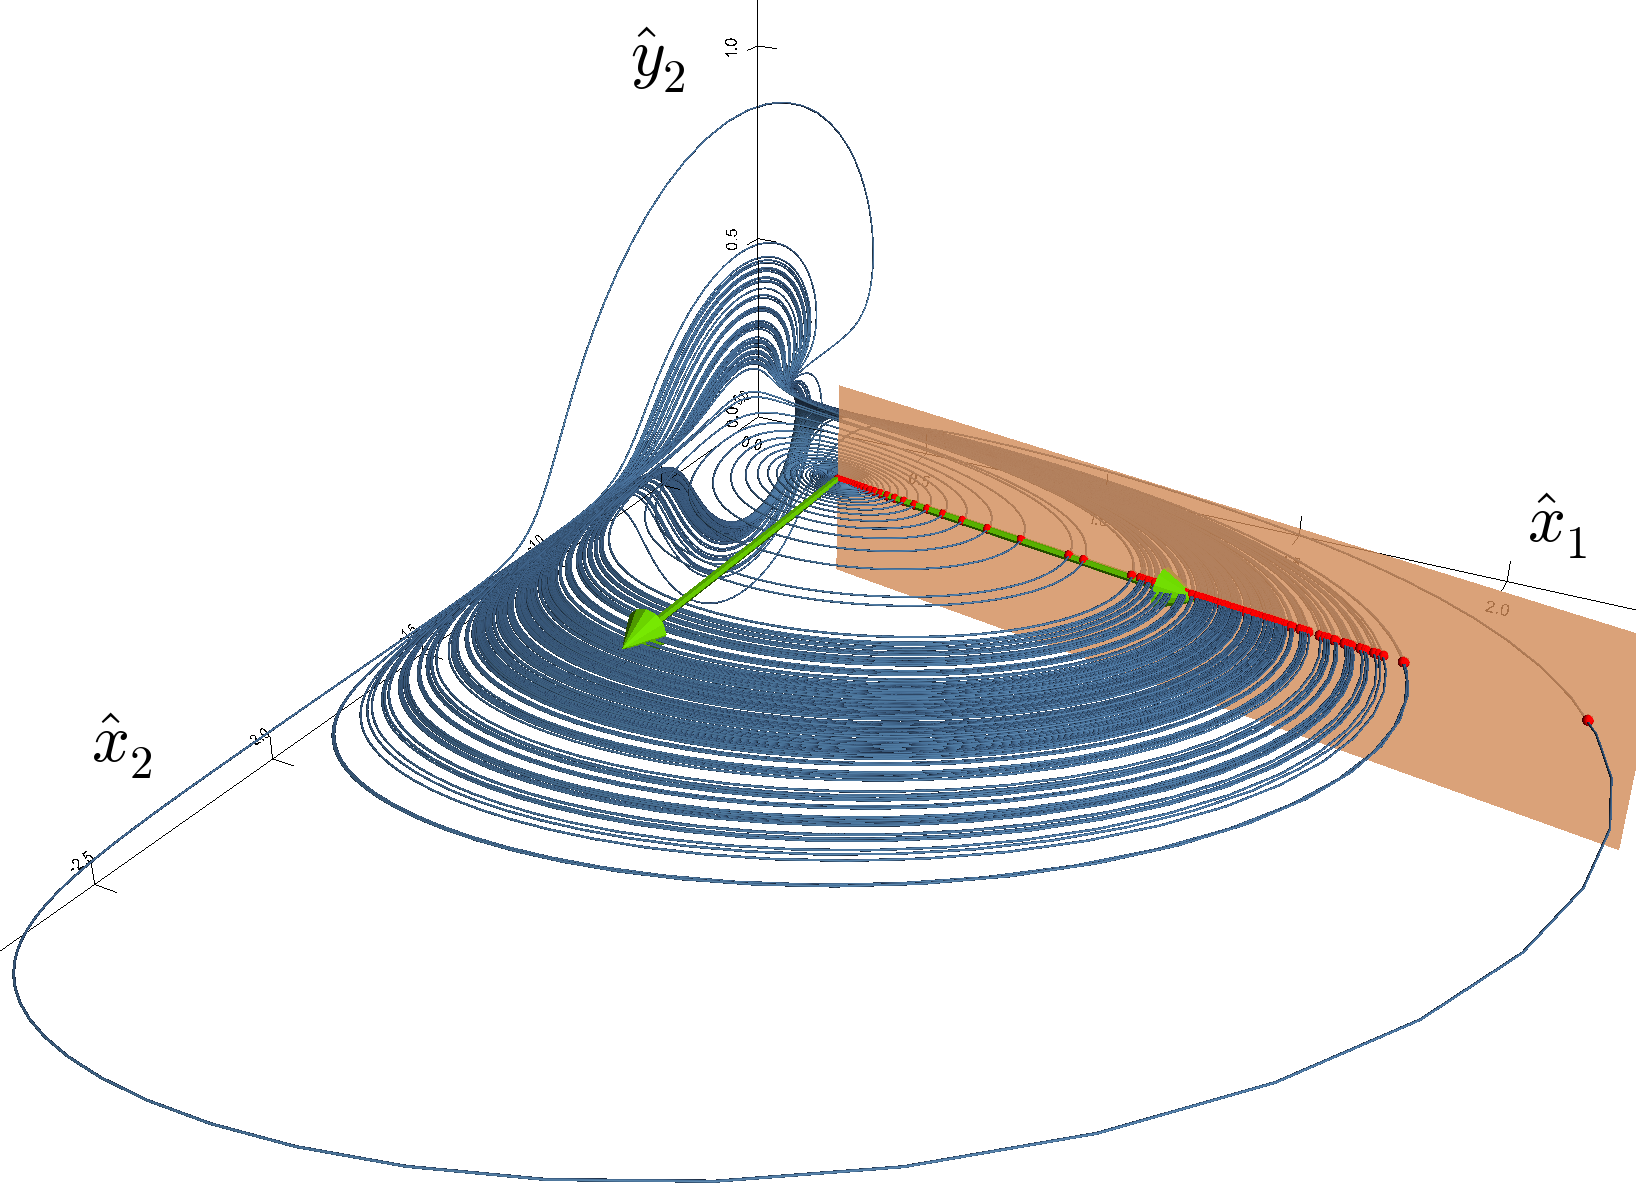
\includegraphics[width=0.45\textwidth]{BBpsecthd} \\
  (b) 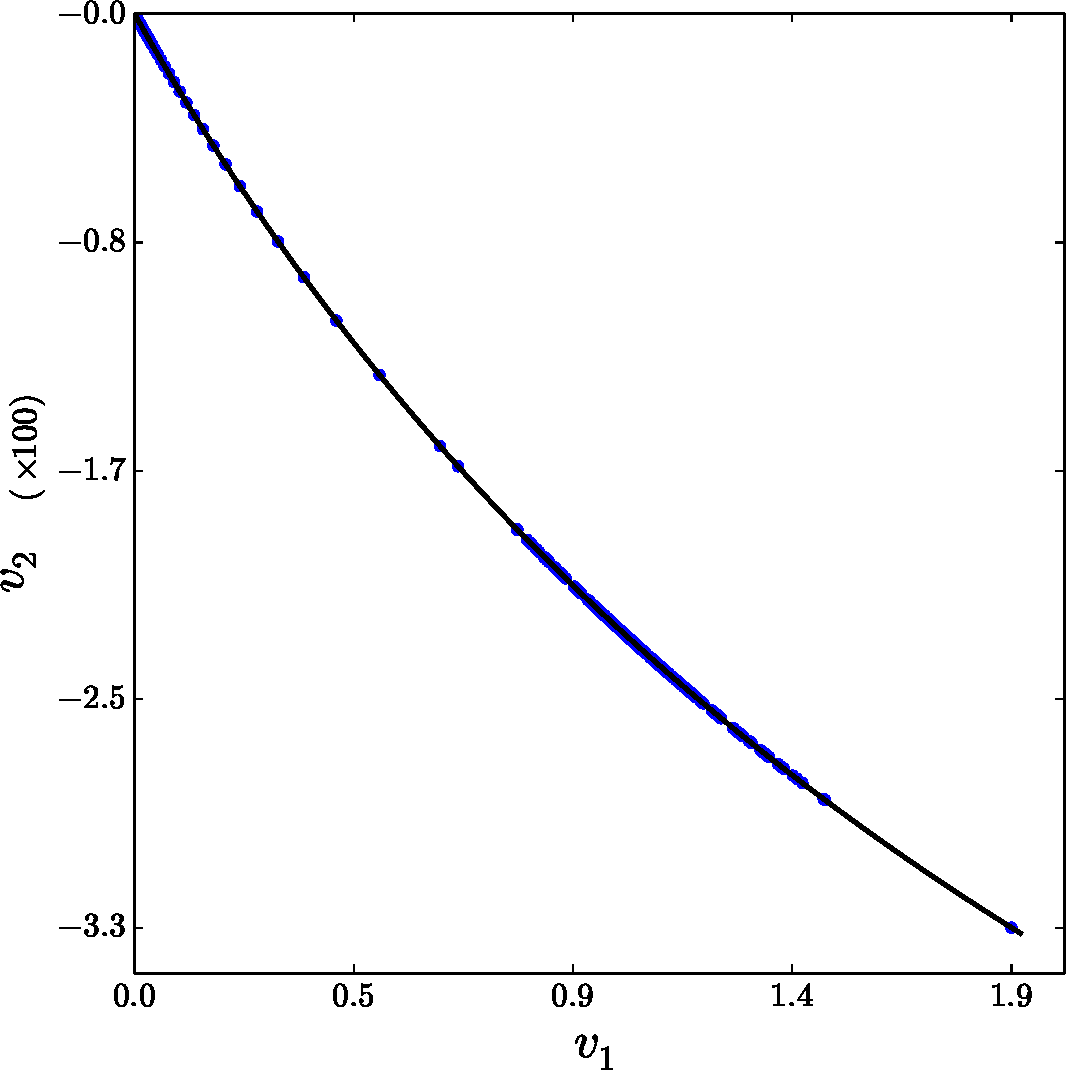
\includegraphics[height=0.19\textwidth]{BBpsectonslice}
  (c) 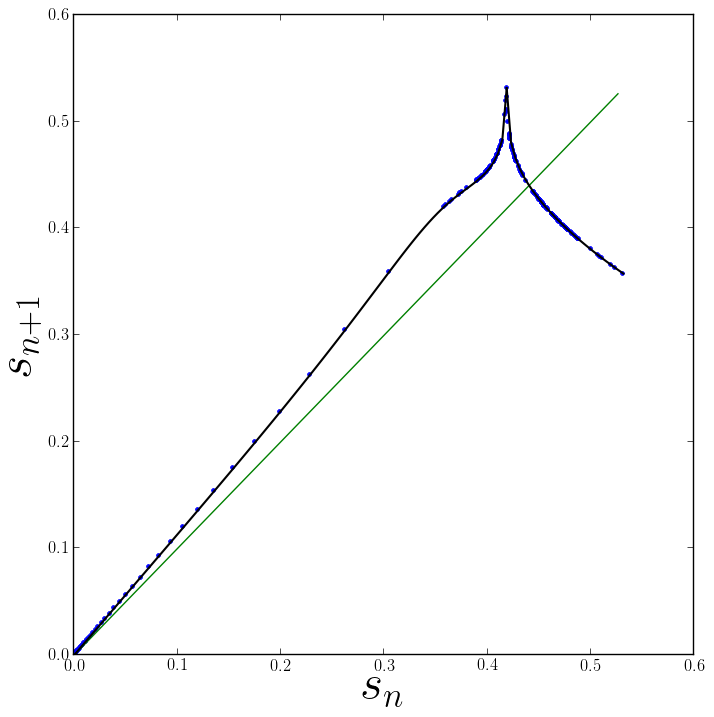
\includegraphics[height=0.19\textwidth]{BBretmaponslice} \\
  (d) 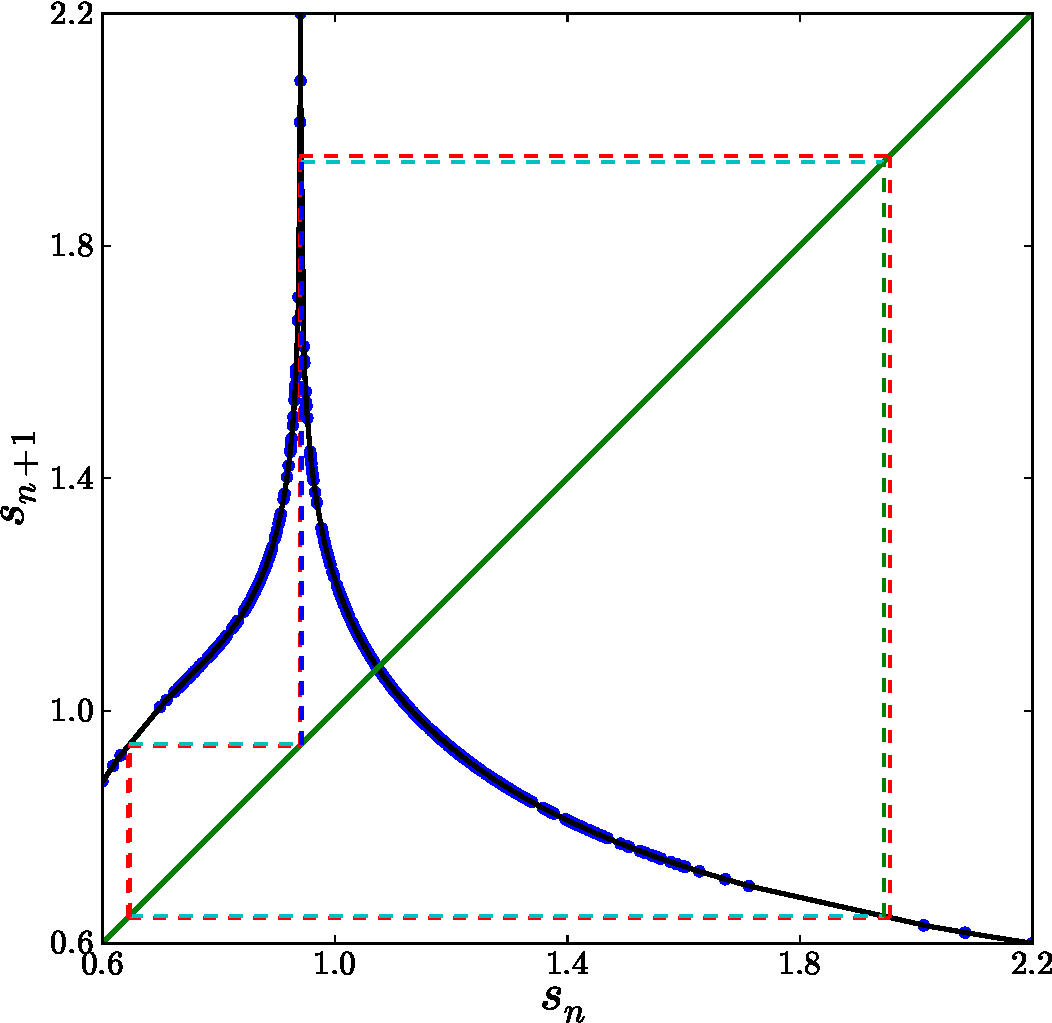
\includegraphics[width=0.45\textwidth]{BBretmaponsliceZoom}
\caption{(a) Symmetry reduced flow within the slice hyperplane (blue).
			Green arrows show the real and imaginary part of the unstable stability
			eigenvector $v_u$ of \REQV{}{}. A Poincar\'e section which includes
			$Im[v_u]$ is visualized as a transparent plane, and sections
			of the flow by the Poincar\'e section are marked with red.
		 (b) The Poincar\'e section which includes the \REQV{}{} and $v_u$ projected
			on to the basis within the plane shown in (a). Included is a
            transient trajectory initiated close to \REQV{}{}. Note that
		  	the vertical axis is magnified by $100$.
		 (c) The Poincar\'e arclength return map for the
		    Poincar\'e section (b).
		 (d) The return map without the transient points, framed by
            orbit of the critical point.
		 	Dashed lines show the 3-cycles \cycle{001} (red) and \cycle{011} (cyan).}
%\ES{on my screen, cyan line appears to change color in vertical parts of the figure.}
%I commented out this edit because it was preventing the file from compiling.
\label{fig:psectandretmap}
\end{figure}

Unimodal return map of \reffig{fig:psectandretmap}\,(d) lets us name the
periodic orbits of the \twomode\ system according to their binary
symbolic dynamics. Critical point of this map is at $s_C=0.98102264$,
corresponding to the tip of the return map. Topological coordinate of the
critical point, the kneading value, lets us determine the all admissible
cycles of the system. For a detailed introduction to the symbolic
dyanmics techniques we refer to \refref{DasBuch}. After determining the
admissible cycles, we find candidates corresponding to the admissible
symbol sequences from the return map, and feed them into a multiple
shooting Newton solver (see Appendix \ref{s:newton}) to precisely
determine the \rpo s. This way, we found the admissible cycles of the
\twomode\ system upto the topological length 12. In
\reffig{f-2modesrpofirst4} we show shortest $4$ of the \rpo s of the
\twomode\ system within the first Fourier mode \slicePlane . As seen from
\reffig{f-2modesrpofirst4}, trajectories of \cycle{001} and \cycle{011}
almost overlap in a large region of the \statesp . This behavior is also
manifested in the return map of \reffig{fig:psectandretmap}\,{d), where
we have shown cycles \cycle{001} and \cycle{011} with red and cyan
respectively. This is a general property of the \twomode\ cycles with odd
topological lengths: They come in pairs with almost equal Floquet
exponents, see \reffig{f-2modes-lambdaDist}.

\begin{figure}%[H]
\centering
 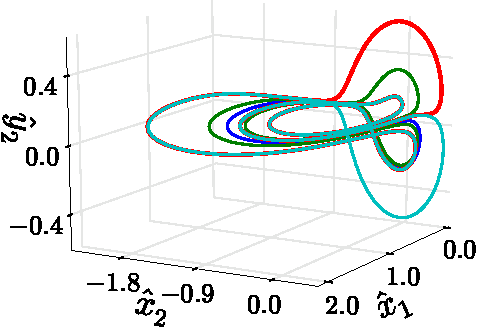
\includegraphics[width=0.45\textwidth]{2modesrpofirst4}
\caption{Shortest four \rpo s of the \twomode\ system: \cycle{1} (dark blue), \cycle{01} (green), \cycle{001} (red), \cycle{011} (cyan). Note that \rpo s \cycle{001} and \cycle{011} almost overlap everywhere except $\hat{x}_1 \approx 0$ .}
\label{f-2modesrpofirst4}
\end{figure}

\begin{figure}%[H]
\centering
 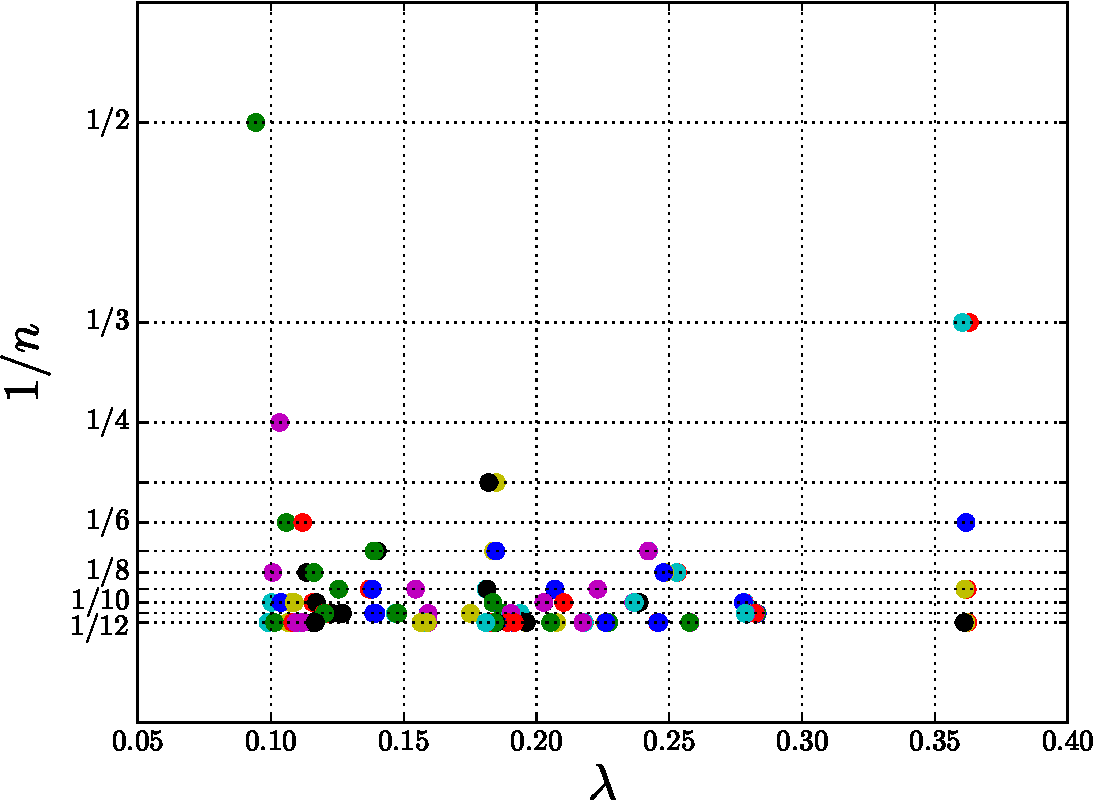
\includegraphics[width=0.45\textwidth]{2modes-lambdaDist}
\caption{Distribution of the leading Floquet exponents of \twomode\ cycles.}
\label{f-2modes-lambdaDist}
\end{figure}

